\title{Homework 6 Solutions for Computer Logic and Circuit Design: PHYS306/COSC330}
\author{Dr. Jordan Hanson - Whittier College Dept. of Physics and Astronomy}
\date{\today}
\documentclass[10pt]{article}
\usepackage[a4paper, total={18cm, 27cm}]{geometry}
\usepackage{graphicx}
\begin{document}
\maketitle

\section{8-2: Types of Shift Register Data IO}

\begin{enumerate}
\item Exercise 6: see Figure \ref{fig:wave0}.
\begin{figure}[ht]
\centering
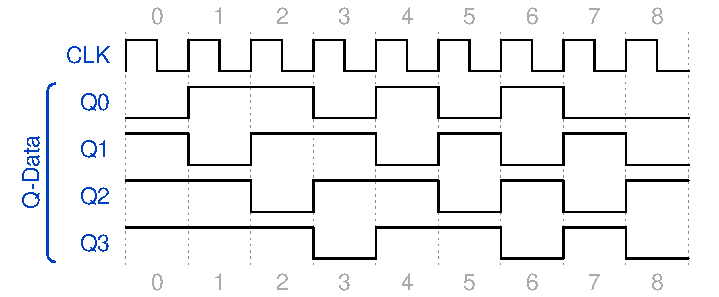
\includegraphics[width=0.5\textwidth]{code/hmk6_8-2-6.pdf}
\caption{\label{fig:wave0} Solution to exercise 6.}
\end{figure}
\item Exercise 8: see Figure \ref{fig:wave1}.
\begin{figure}[ht]
\centering
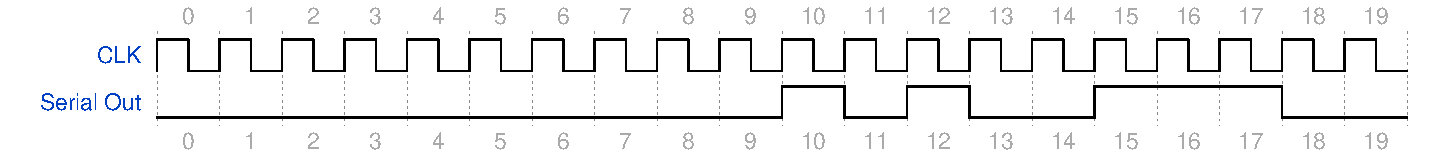
\includegraphics[width=0.9\textwidth]{code/hmk6_8-2-8.pdf}
\caption{\label{fig:wave1} Solution to exercise 8.}
\end{figure}
\item Exercise 10: 11011010, which is 218.
\item Exercise 14: see Figure \ref{fig:wave2a}.
\begin{figure}[ht]
\centering
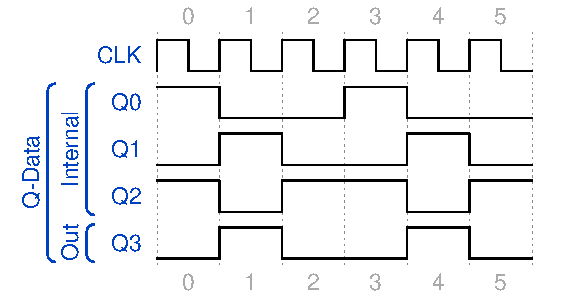
\includegraphics[width=0.5\textwidth]{code/hmk6_8-2-14.pdf}
\caption{\label{fig:wave2a} Solution to exercise 14.}
\end{figure}
\end{enumerate}

\section{8-3: Bidirectional Shift Registers}

\begin{enumerate}
\item Exercise 21: see Figure \ref{fig:wave2}.
\begin{figure}[ht]
\centering
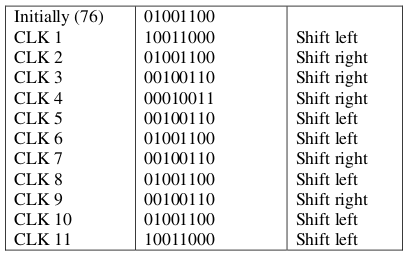
\includegraphics[width=0.5\textwidth]{code/exercise21.png}
\caption{\label{fig:wave2} Solution to exercise 21.}
\end{figure}
\end{enumerate}

\section{8-4: Shift Register Counters}

\begin{enumerate}
\item Exercise 28: see Figure \ref{fig:wave3}.
\begin{figure}
\centering
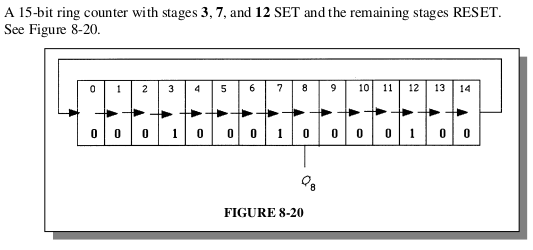
\includegraphics[width=0.75\textwidth]{code/exercise28.png}
\caption{\label{fig:wave3} Solution to exercise 28.}
\end{figure}
\end{enumerate}

\end{document}